\chapter{Results}

\section{Goals}
We want to look at the effect that extending a KG has on the rules mined from it and the effect of different factors in the KG extension process. Will new correct rules be mined when the KG is extended with facts deemed plausible by a KG embedding? Are these new rules of the same quality as rules mined from the original KG. Will all the original rules also be mined from the extended KG? Furthermore we want to evaluate the effect of parameter choice when extending the KG, namely the KG embedding model architecture, the entity selection method and rank cutoff.

\section{Overview of results}

\subsection{KG extension sizes}
In the KG extension process there are 48 different parameter combinations. This means that there are 48 different KG extensions for each original KG. Extension set sizes ranged from around 800 to 33500 triples, where the RandomBaseline model admitted the most candidates. This makes sense, as the models assigns a random score to triples resulting in many more triples receiving a high rank. The other trained models give most candidates a low score because most triples are bad candidates. Note that the extension sizes were about the same for both datasets, while WN18RR and the family KG respectively have 88 227 and 258 235 facts, therefore the extensions for WN18RR are relatively larger than for the family KG.

\subsection{Rule set sizes and mean PCA confidence}
When examining the number of rules mined in each KG extension one immediately sees some startling results. Most rule sets don't differ drastically in size apart from those where TransE was used, where these rule sets are exceptionally larger. See figure X and Y (TODO: add figures) in the appendix to observe the difference. When looking at the mean PCA confidence of the rules sets one also notes that the score for the TransE sets are mostly around 0.1, while the remaining rule sets have a score on average around 0.5.

\begin{figure}[h]
\centering
\begin{subfigure}{.5\textwidth}
  \centering
  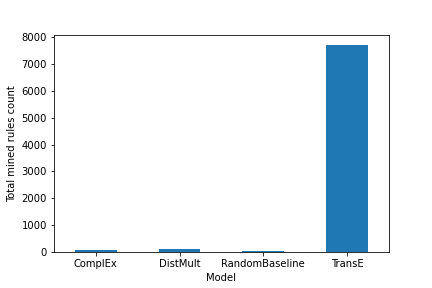
\includegraphics[width=1\linewidth]{figures/results/Total_mined_rules-model-wn18rr.png}
  \caption{WN18RR}
  \label{fig:sub1}
\end{subfigure}%
\begin{subfigure}{.5\textwidth}
  \centering
  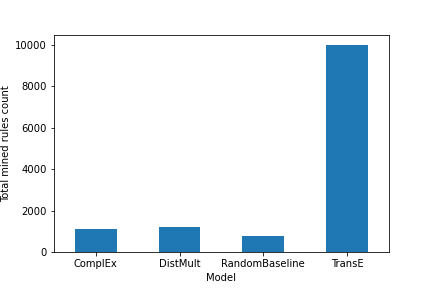
\includegraphics[width=1\linewidth]{figures/results/Total_mined_rules-model-family.png}
  \caption{Family KG}
  \label{fig:sub2}
\end{subfigure}
\caption{Distribution of number of mined rules over different embedding models.}
\label{fig:test}
\end{figure}

As discussed in (TODO: add section) TransE is not able to learn some type of relations, and upon further inspection of the embedding vectors for relations in TransE the vector values all tend toward zero. It seems that while scoring decently on the performance metrics during model selection, TransE has not properly embedded the relations in the KG. Of the rules mined, 97\% (WN18RR) and 76\% (family KG) come from KGs extended using TransE. Due to the fact that the trained TransE model has poor relational embeddings and that the large number of rules produced from this overshadow the rules mined using other embedding models, we will include  rules mined from KGs when examining embedding models, but not consider these datapoints when looking at entity selection methods or rank cutoff criteria.

\section{Effect of parameters}
\subsection{Effect of KG embedding model}

\begin{table}[h]
\begin{tabular}{|l|ccc||ccc|}
\hline
{\textbf{DATASET}}   & \multicolumn{3}{c||}{\textbf{WN18RR}}                                                                              & \multicolumn{3}{c|}{\textbf{Family KG}}                                                           \\ \hline
{\textbf{RULE GROUPS}}   & \multicolumn{1}{c|}{\textbf{Not found}} & \multicolumn{1}{c|}{\textbf{Found}} & \multicolumn{1}{c||}{\textbf{New}} & \multicolumn{1}{c|}{\textbf{Not found}} & \multicolumn{1}{c|}{\textbf{Found}} & \multicolumn{1}{c|}{\textbf{New}} \\ \hline
\textbf{ComplEx}  & \multicolumn{1}{c|}{0}                  & \multicolumn{1}{c|}{10}             & \multicolumn{1}{c||}{19}           & \multicolumn{1}{c|}{0}                  & \multicolumn{1}{c|}{94}             & \multicolumn{1}{c|}{73}           \\ \hline
\textbf{DistMult} & \multicolumn{1}{c|}{0}                     & \multicolumn{1}{c|}{10}                                  & 16                                & \multicolumn{1}{c|}{1}         & \multicolumn{1}{c|}{93}          & 115                               \\ \hline
\textbf{TransE}   & \multicolumn{1}{c|}{0}         & \multicolumn{1}{c|}{10}                     & 811                               & \multicolumn{1}{c|}{7}       & \multicolumn{1}{c|}{87}      & 1083                              \\ \hline
\textbf{Baseline} & \multicolumn{1}{c|}{1}     & \multicolumn{1}{c|}{9}                   & 0                                 & \multicolumn{1}{c|}{12}       & \multicolumn{1}{c|}{82}         & 16                                \\ \hline
\end{tabular}
\caption{Overview of which KG embedding models found all the original rules and how many new rules were found.}
\end{table}


    \begin{figure*}[h]
        \centering
        \begin{subfigure}[b]{0.49\textwidth}
            \centering
            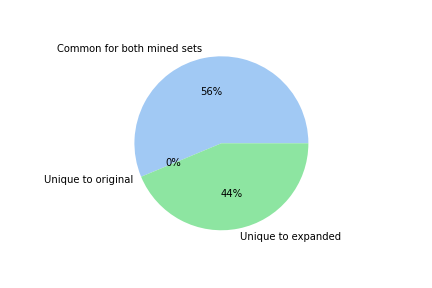
\includegraphics[width=\textwidth]{figures/results/pie_charts-model/complEx_family.png}
            \caption[complEx_pie]%
            {{\small ComplEx}}    
            \label{fig:complex_pie}
        \end{subfigure}
        \hfill
        \begin{subfigure}[b]{0.49\textwidth}  
            \centering 
            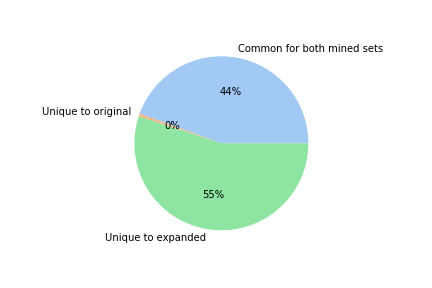
\includegraphics[width=\textwidth]{figures/results/pie_charts-model/distMult_family.png}
            \caption[]%
            {{\small DistMult}}    
            \label{fig:distMult_ppie}
        \end{subfigure}
        \vskip\baselineskip
        \begin{subfigure}[b]{0.49\textwidth}   
            \centering 
            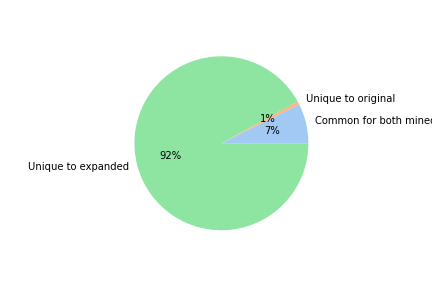
\includegraphics[width=\textwidth]{figures/results/pie_charts-model/transE_family.png}
            \caption[]%
            {{\small TransE}}    
            \label{fig:trasE_pie}
        \end{subfigure}
        \hfill
        \begin{subfigure}[b]{0.49\textwidth}   
            \centering 
            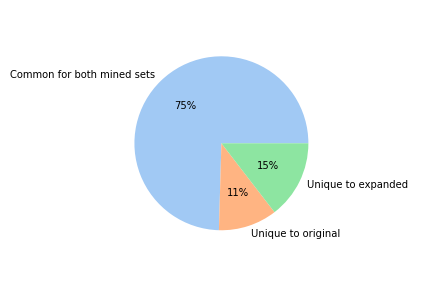
\includegraphics[width=\textwidth]{figures/results/pie_charts-model/randomBaseline_family.png}
            \caption[]%
            {{\small RandomBaseline}}    
            \label{fig:randomBaseline_pie}
        \end{subfigure}
        \caption[ The average and standard deviation of critical parameters ]
        {\small Distribution of all the rules mined over KG embedding models. KG: family KG.} 
        \label{fig:mean and std of nets}
    \end{figure*}
    
    
    \begin{figure*}[h]
        \centering
        \begin{subfigure}[b]{0.49\textwidth}
            \centering
            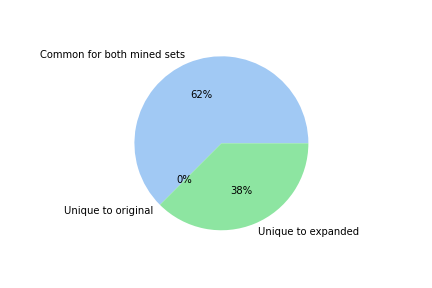
\includegraphics[width=\textwidth]{figures/results/pie_charts-model/complEx_wn18rr.png}
            \caption[complEx_pie]%
            {{\small ComplEx}}    
            \label{fig:complex_pie}
        \end{subfigure}
        \hfill
        \begin{subfigure}[b]{0.49\textwidth}  
            \centering 
            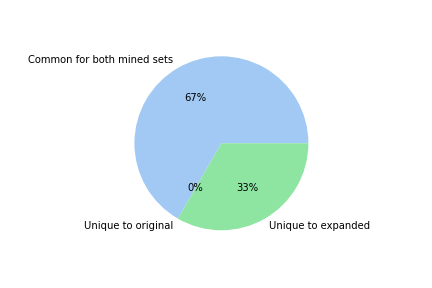
\includegraphics[width=\textwidth]{figures/results/pie_charts-model/distMult_wn18rr.png}
            \caption[]%
            {{\small DistMult}}    
            \label{fig:distMult_ppie}
        \end{subfigure}
        \vskip\baselineskip
        \begin{subfigure}[b]{0.49\textwidth}   
            \centering 
            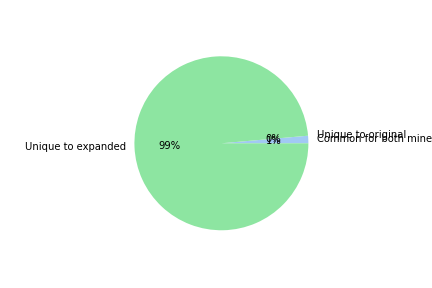
\includegraphics[width=\textwidth]{figures/results/pie_charts-model/transE_wn18rr.png}
            \caption[]%
            {{\small TransE}}    
            \label{fig:trasE_pie}
        \end{subfigure}
        \hfill
        \begin{subfigure}[b]{0.49\textwidth}   
            \centering 
            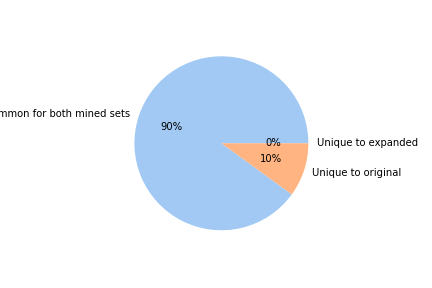
\includegraphics[width=\textwidth]{figures/results/pie_charts-model/randomBaseline_wn18rr.png}
            \caption[]%
            {{\small RandomBaseline}}    
            \label{fig:randomBaseline_pie}
        \end{subfigure}
        \caption[ The average and standard deviation of critical parameters ]
        {\small Distribution of all the rules mined over KG embedding models. KG: WN18RR.} 
        \label{fig:mean and std of nets}
    \end{figure*}
    
    
    
\begin{figure}[h]
\centering
\begin{subfigure}{.5\textwidth}
  \centering
  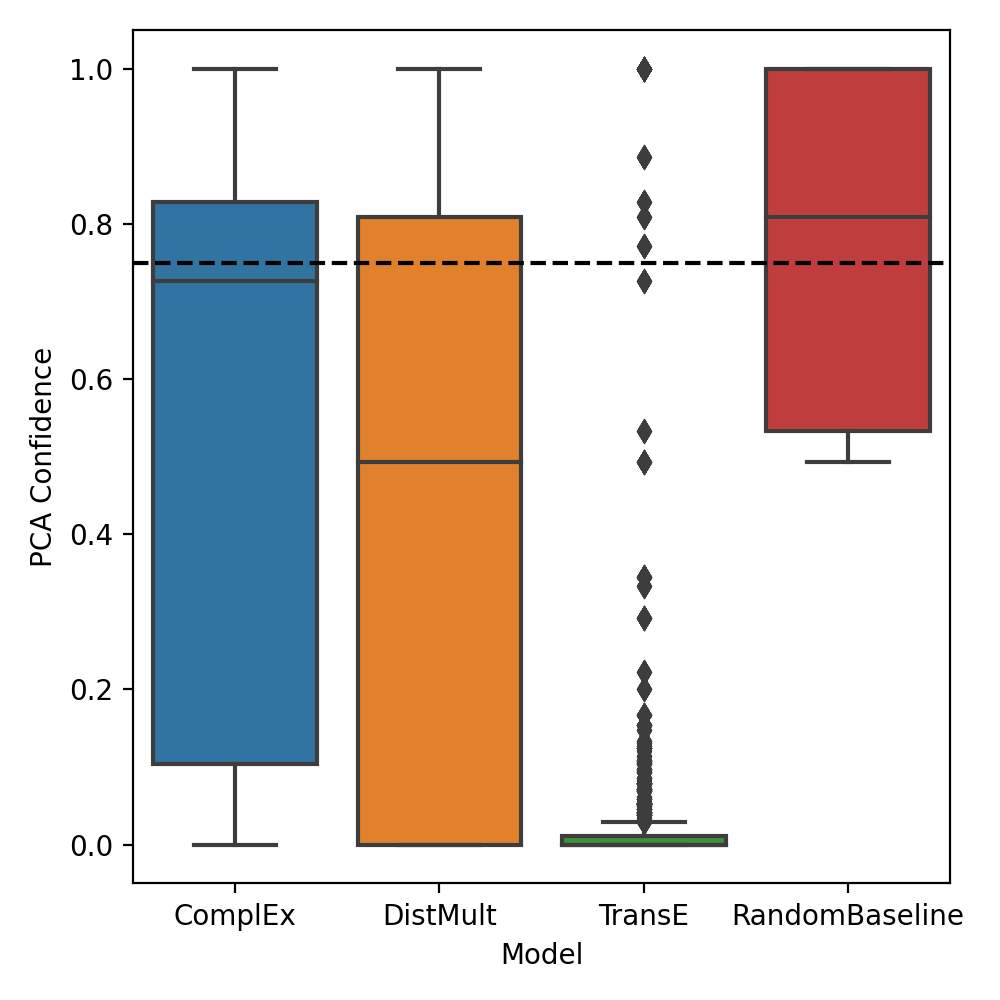
\includegraphics[width=1\linewidth]{figures/results/PCA_models/PCA-models_wn18rr.png}
  \caption{Original KG}
  \label{fig:PCA-models_wn18rr_boxplot_sub}
\end{subfigure}%
\begin{subfigure}{.5\textwidth}
  \centering
  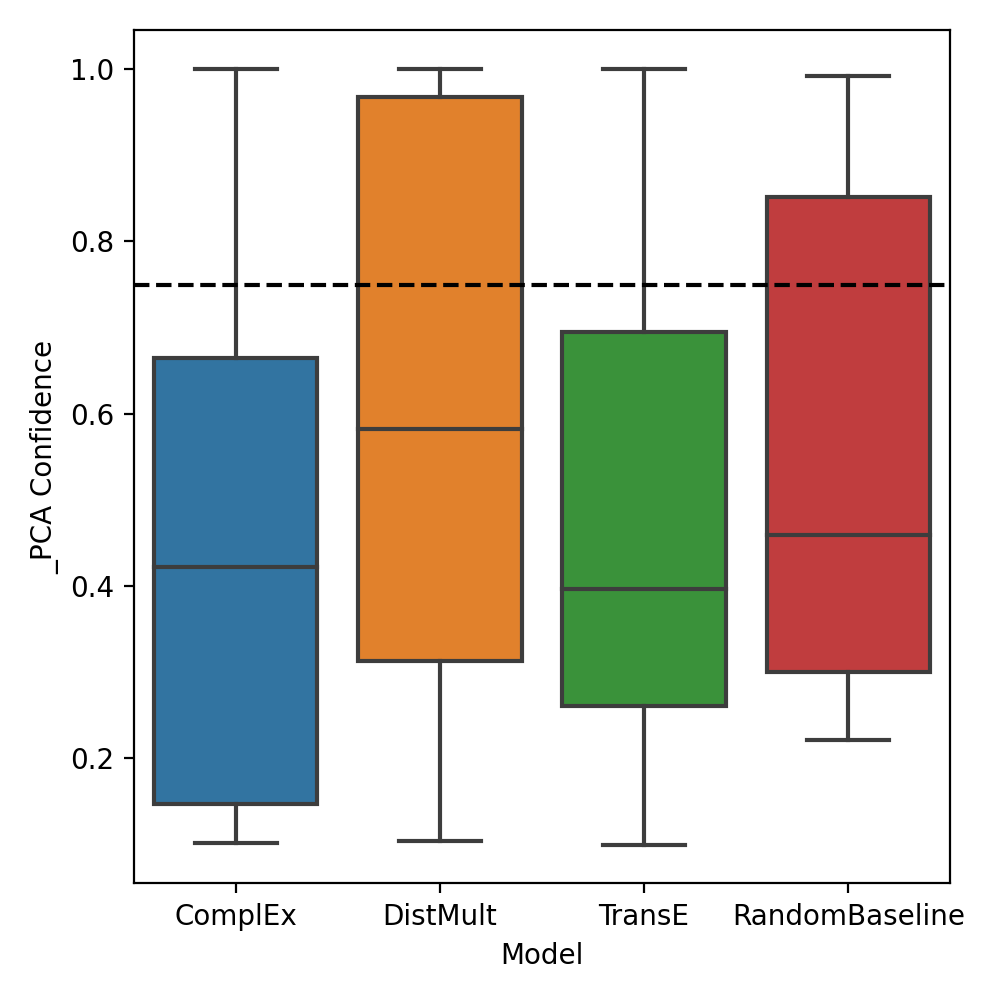
\includegraphics[width=1\linewidth]{figures/results/PCA_models/_PCA-models_wn18rr.png}
  \caption{Extended KG}
  \label{fig:_PCA_models_wn18rr_boxplot_sub}
\end{subfigure}
\caption{Distribution of PCA confidence of mined rules by KG embedding models. PCA confidence scores are calculated on the original WN18RR and the extended WN18RR from which the rules are mined. The dashed line represents the median PCA confidence of the rules mined from the original WN18RR KG.}
\label{fig:test}
\end{figure}

\begin{figure}[h]
\centering
\begin{subfigure}{.5\textwidth}
  \centering
  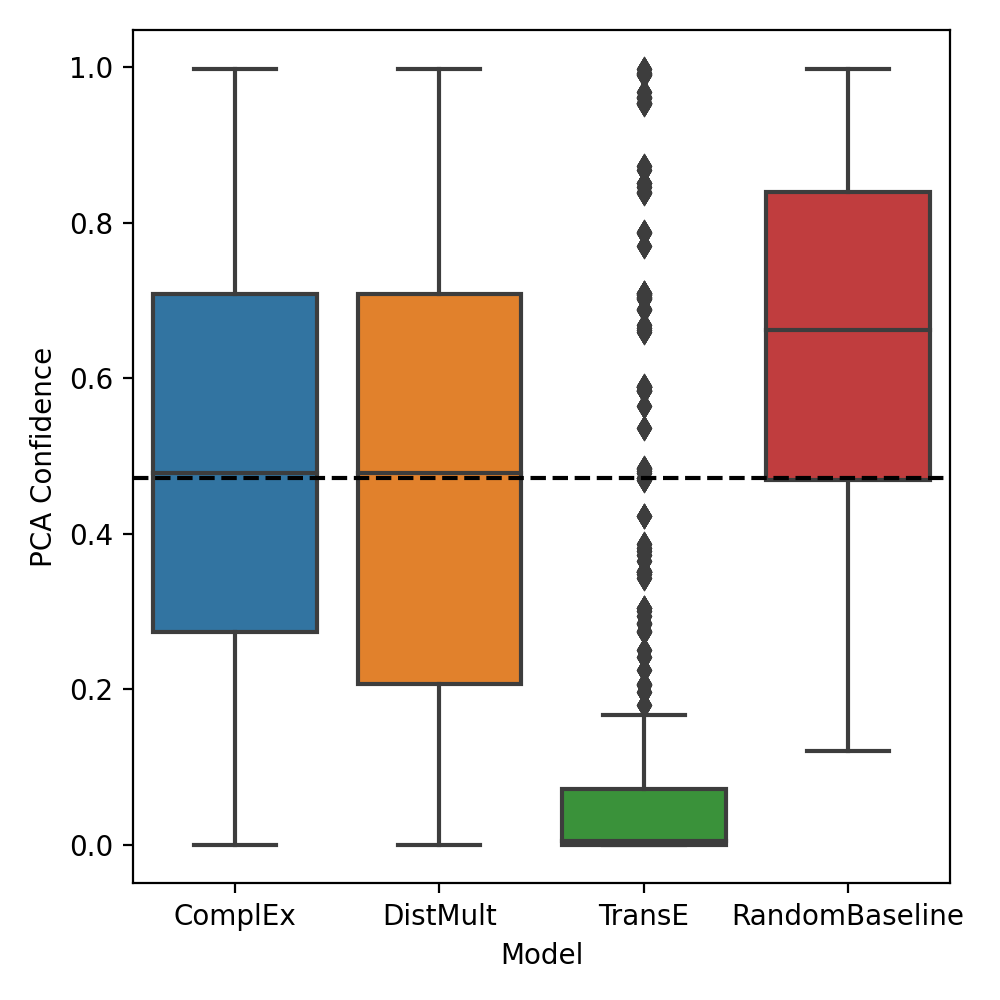
\includegraphics[width=1\linewidth]{figures/results/PCA_models/PCA-models_family.png}
  \caption{Original KG}
  \label{fig:models_family_boxplot_sub}
\end{subfigure}%
\begin{subfigure}{.5\textwidth}
  \centering
  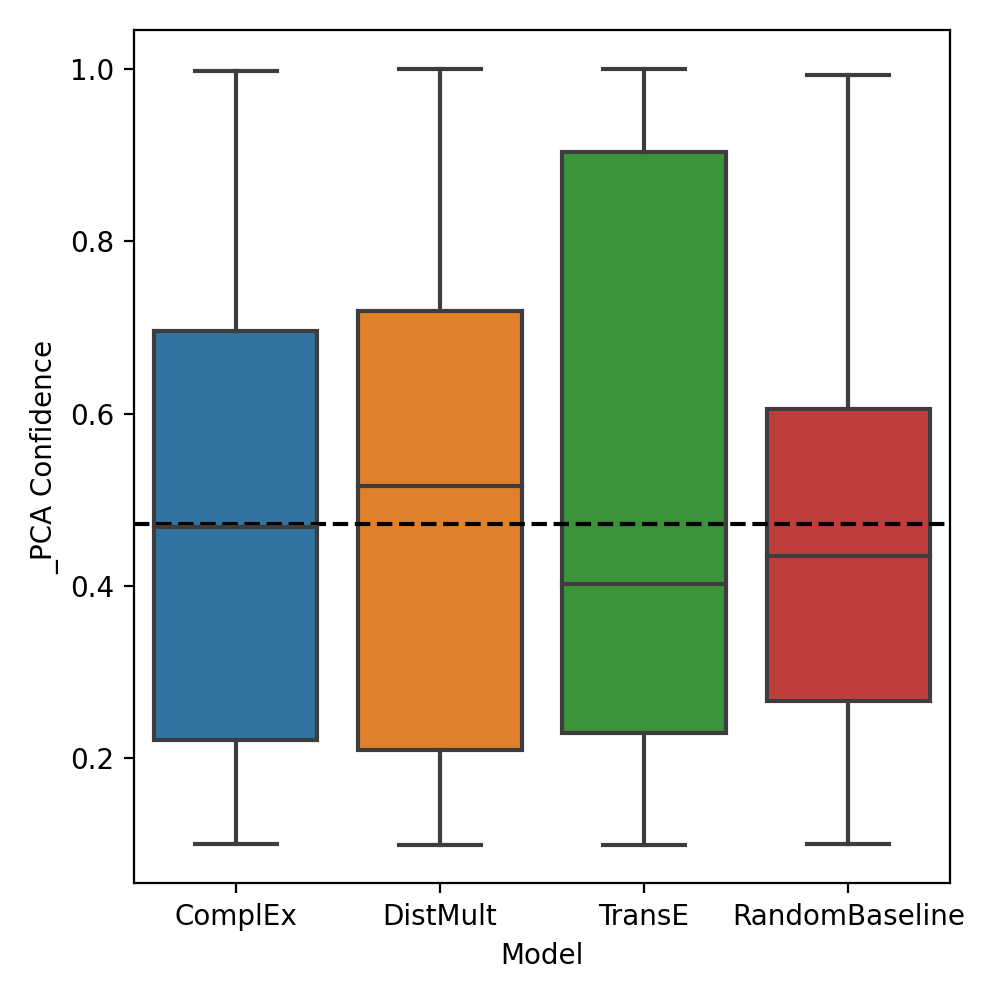
\includegraphics[width=1\linewidth]{figures/results/PCA_models/_PCA-models_family.png}
  \caption{Extended KG}
  \label{fig:_PCA_models_family_boxplot_sub}
\end{subfigure}
\caption{Distribution of PCA confidence of mined rules by KG embedding models. PCA confidence scores are calculated on the original family KG and the extended family KG from which the rules are mined. The dashed line represents the median PCA confidence of the rules mined from the original family KG.}
\label{fig:PCA_models_family_boxplot}
\end{figure}

\subsection{Effect of entity selection method}

\subsection{Effect of rank cutoff value}